\documentclass[11pt]{article}   	% use "amsart" instead of "article" for AMSLaTeX format
\usepackage[margin=2cm]{geometry}

\usepackage{graphicx}				% Use pdf, png, jpg, or eps§ with pdflatex; use eps in DVI mode
								% TeX will automatically convert eps --> pdf in pdflatex		
%\usepackage{amssymb}
\usepackage{float} % formats figures
\usepackage{fancyhdr}
\usepackage{hyperref} % create clickable links
\pagestyle{fancy}
 \usepackage{setspace}
\lhead{Student: Lina Rietuma}
\cfoot{\thepage}
\rhead{ID: H00361943}

% No paragraph indentation
\setlength\parindent{0pt}
\setlength\parskip{1em}
\raggedright

\setstretch{1.25}

\begin{document}

\begin{center}
  \Huge{F21DV Lab 1 Report}
\end{center}
Date: 28/01/2022 \linebreak
Demonstrated To: Shuangjiang  Xue \linebreak
Repository: \url{https://github.com/linarietuma/linarietuma.github.io} 

\section{Introduction}

This report summarises the reflections and results of exercises for Data Visualisations and Analytics (F21DV) course Lab 1. The code is organised in parts each part corresponding to a separate HTML file which can be accessed from the main index.html. The code is maintained in a GitHub repository and accessible using GitHub pages.

\section{Part 2: D3 Setup}
\subsection{Exercise 1: What version number is displayed in the console output window?}
\vspace{-1em}

D3 version number displayed is 7.3.0.

\subsection{Exercise 2 }
\vspace{-1em}

Exercise 2 required changing the style properties of the paragraph tag. Function .select("p") is used to select the first HTML element (e.g., div, p, \#id, .class) of the specified type and .style("color", "red") to format the selected element where the first argument specifies CSS property and the second argument denotes its value. Additional style properties added include transforming text to uppercase and adding underline text decoration

\subsection{Exercise 3 }
\vspace{-1em}

Exercise 3 required adding 10 'div' elements containing values from 1 to 10 in a loop and colouring each element based on its index. 
Both .style() and .attr() methods are used in combination with the .select()/ .selectAll() methods to change the properties of the specified element/s. While .style() is used to change CSS styling, . attr() changes an attribute of the selected element (e.g. set class, id etc).

\subsection{Exercise 4 }
\vspace{-1em}
Exercise 4 builds on exercise 3 and requires selecting and modifying the 'div' elements after they've been created. When creating the elements, each is given a unique id which later allows to specifically target and change the desired elements using select(), style () and text () functions.  

\subsection{Exercise 5 }
\vspace{-1em}
Exercise 5 required modifying the sample code to demonstrate the 'chain syntax' by changing the text colour.
In D3, methods can be chained together to avoid storing intermediary variables that are passed between methods. The colour of the text is changed using the style() function to select the colour attribute and set it to purple.


\section{Part 3: Data}
\subsection{Exercise 6 }
\vspace{-1em}
Exercise 6 build on the sample code to add an additional 'color' variable to the array of JSON objects and print it.
Function data() is used to select and iterate through the data, allowing to access and modify values one by one. 'color' key-value pair is added to each object in the data array and retrieved by calling d.color.

\subsection{Exercise 7 }
\vspace{-1em}
Exercise 7 build on the sample code to change the colour of a data point based on its value - red for numbers between 50 and 100 (assumed this includes the boundary values). To achieve this, if statement within the style() function is update to have 100 as the upper bound and include 50 as the lower bound.

\section{Part 4: Data Binding}
\subsection{Exercise 8 }
\vspace{-1em}
Exercise 8 builds on the sample code and required setting the colour of a data point based on its type - blue if it's a character, green if it's a number. Function data() is used for data selection and enter() to bind data to a specific HTML element. If no element of the specified type is found, enter() creates the element and append() adds it to the page.

A lot of D3 methods will accept a function as an argument (e.g. text(), style(), etc), this functionality allows changing properties of an element based on the data value. For this exercise, a function is parsed to set the colour attribute and typeof operator is used to determine the type of a data value.


\section{Part 5: Loading Data}
\subsection{Exercise 9 }
\vspace{-1em}
Exercise 9 required processing the Titanic sample data to determine the number of passenger names that include 'Mr.' and 'Mrs' (or other) and additional information from the data.  A CSV file is read in using the csv() function which accepts a CSV file path and a callback function as arguments. Within the callback function, each CSV line is individually processed and the required information is captured using pre-defined variables. 

The csv() function is asynchronous to prevent the page from freezing up while data are being processed therefore to ensure all data are processed before any further functions are called, the request from the csv() is saved in a variable. To determine when the request is fulfilled, then() function is executed which contains several console.log() statements to print the processed data - the number of passengers with 'Mr.' and 'Mrs' in their name, the number of females and males, and the average age of Titanic's passengers.


\subsection{Exercise 10 }
\vspace{-1em}
Exercise 10 builds on the sample code provided and required additional pre-processing of the heart failure data to display heart failures in age ranges 1-30, 31-40, 41-60 and 61-100. Similarly to exercise 9, data are loaded from an external CSV file using the csv() function, processed within the callback function and added to screen within the then() function. 


\section{Part 6: SVG}
\subsection{Exercise 11 }
\vspace{-1em}
Exercise 11 introduced SVG elements and required creating a square from four separate line objects. SVG functions as a container to more easily display visual  information. Each line is added to the SVG using the append() function with the position and length of the line specified through x1, x2, y1, y2 attributes. To create a square, each subsequent line must start were the previous line ended, and be rotated by 90 degrees. Colour of the lines are set through the stroke attribute.

\subsection{Exercise 12 }
\vspace{-1em}
Exercise 12 required adding different shapes to the page based on data from a CSV file which include information about the type, size, position and colour of the shape. The CSV contains a line per shape with the first column specifying the shape type and the rest indicating size, position and colour attributes of all basic shapes (e.g. height, width, cx, cy, r etc.) with the irrelevant columns for each shape left empty (e.g. 'r' is left empty for a rectangle, 'height' for a circle etc.).  Data are loaded using the csv() and processed within the callback function which contains a switch statement to call the relevant attributes based on a shape's type and append the elements to a pre-defined SVG object..

\subsection{ Exercise 13 }
\vspace{-1em}
Exercise 13 builds on exercise 12 to include enter() and exit() concepts. To demonstrate these concepts, ten additional circles are added to the SVG prior to loading the data from a CSV. Within the csv() callback function fill colours of each shape are saved in array and shapes are added to the page based on the parameters defined in the external file. 

Once the SVG scene is created, all circle elements are selected (11 in total) and data() is called with the array of colors as an argument (5 in total). The data() function iterates through each data point within the array and calls either enter(), update() or exit() functions. Since there are more circle elements than data points in the array, enter() function is never called, update() function is called for the first five circle elements and their colour changed, and the exit() function is called for the rest of the circle elements which are removed (including the circle created from the CSV data).  

Similarly, all rectangle objects are selected, however in this case enter() function is called to add additional elements.


\section{Part 7: Bar Chart}
\subsection{Exercise 14 }
\vspace{-1em}
Exercise 14 required displaying a bar chart with heart failure data from Part 5. The data are saved in a 2D array as key-value pairs where key is the data label. For each value, a container element 'g' is added to the page using the data(), enter() and append() functions. Each container is repositioned using the indices of the datapoints and appended a rectangle object, the width of which is dependant on the data value. Similarly the data labels are added to the container and positioned using the data values.   

\subsection{Exercise 15 }
\vspace{-1em}
Exercise 15 required modifying the bar chart from exercise 14 to include additional colour elements. The colour of the bars is determined from the data values through a series of if statements passed as a function with the attr() function (Figure \ref{fig:ex15}). 

\begin{figure}[H]
\centering
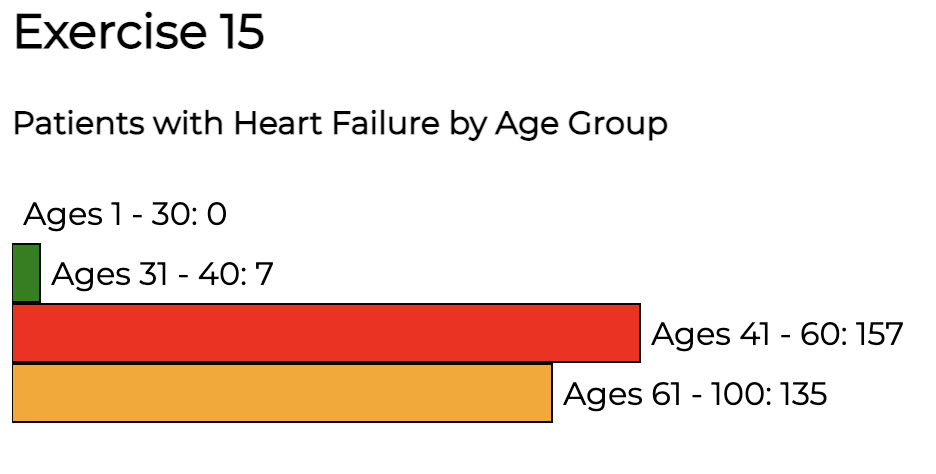
\includegraphics[width=0.65\textwidth]{data/ex15.png}
\caption{A bar chart with bars' colour dependant on the data value.}
\label{fig:ex15}
\end{figure}

\section{Part 8: Circle Chart}
\subsection{Exercise 16 }
\vspace{-1em}
Exercise 16 required adding additional shapes (e.g. circles and rectangles) to the sample code. A container element is added for each value in the data array and append() function is called to add 'rect' and 'circle' elements. The size, colour and position properties are set using the attr() functions that are linked together using chain syntax. 


\section{ Part 9: Scales, Domain, Range }
\subsection{Exercise 17 }
\vspace{-1em}
Exercise 17 required modifying the sample bar chart code to set a bar colour to green if a data value is below 100 and red if it's above 500. Similarly to exercise 15, the colour of the bars is determined through a series of if statements within the attr() function that sets the fill colour. To ensure the bar chart fits within the bounds of the SVG object, scaleLinear() function is used to scale values within the domain (set using the domain() function) to values within the given range (set using the range() function). 

\subsection{ Exercise 18 }
\vspace{-1em}
Exercise 18 required displaying a bar chart with data read in from a CSV file. The code from exercise is reused with the data array read in from a CSV using csv() function and the bar chart built within the then() function.

\subsection{ Exercise 19 }
\vspace{-1em}
Exercise 19 required to encapsulate the bar chart sample code in a function which appends a bar chart to the page from the data provided. The given code is separated in two function - createBarChart() and createChart(). The first function accepts a data array as an argument which is used to create a bar chart and append to page. The second function determines the data sources that is passed to the createBarChart() function. As an optional argument, the createChart() function accepts a path to CSV file to load data from file, if the argument is omitted a default data array is created to be used in the createBarChart().

\section{Part 10: Axis}
\subsection{Exercise 20 }
\vspace{-1em}
Exercise 20 required updating the sample code to add an additional blue axis at the top and on the right. Axes objects are created using axisRight() and axisTop() functions, and the distribution of tick markers are set using the scale() function.

\subsection{Exercise 21 }
\vspace{-1em}
Exercise 21 required adding and x and y axis to a bar chart. The bar chart from exercise 17 is used. The x axis uses the same linear scale as the bars while the y axis contains discrete values therefore scaleOrdinal() function is used (Figure \ref{fig:ex21}). 

\begin{figure}[H]
\centering
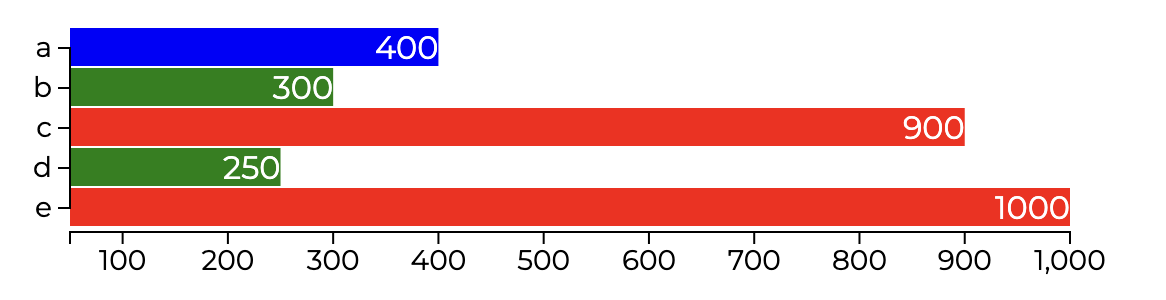
\includegraphics[width=0.75\textwidth]{data/ex21.png}
\caption{A bar chart with a linear x axis and an ordinal y axis.}
\label{fig:ex21}
\end{figure}

\section{Part 12: Line Chart }
\subsection{ Exercise 22 }
\vspace{-1em}
Exercise 22 required encapsulating the sample line chart code within a function. The function created accepts a data array as argument and optionally the name of the HTML element the chart must be appended to (for the purposes of organising code). 

\subsection{Exercise 23 }
\vspace{-1em}
Exercise 23 required loading data from an external source and plotting the data on a line chart. Data are loaded from CSV file using csv() function and saved within an array. The function from exercise 22 is called within the then() function and the CSV data array is passed as an argument. 

\subsection{ Exercise 24 }
\vspace{-1em}
Exercise 24 required adding multiple differently coloured lines to the same chart in blue and green. Two data arrays are generated using the Math.sin() and Math.cos() functions. To determine the scale of the graph, a function findExtent() is created which accepts the min and max values (i.e. the extent) of each data array and determines the combination of values that would create a domain to cover all the data values. Each line is added to the chart as a separate path the coordinates of which are determined using the line() function. 

\section{Part 13: Markers}
\subsection{Exercise 25 }
\vspace{-1em}
Exercise 25 required adding a circle marker to each data point on a line chart. In essence, adding small circle shapes, the position of which is dependant on the data values. 


\subsection{ Exercise 26 }
\vspace{-1em}
Exercise 26 required plotting two lines on a single chart, each with different markers - circles and triangles respectively. Circles are basic shapes within D3, therefore can be easily added using the data array to position the markers. On the other hand triangles are not one of the basic shapes in D3, therefore a polygon shape is added with three defined points, the position of which are again dependant on the data array. The colour of the markers is set using the fill attribute.



\subsection{Exercise 27 }
\vspace{-1em}
Exercise 27 required adding data labels to the markers on a line chart. To prevent the text from overcrowding the chart, a label is added to every 9th data point using indices (Figure \ref{fig:ex27}). 

\begin{figure}[H]
\centering
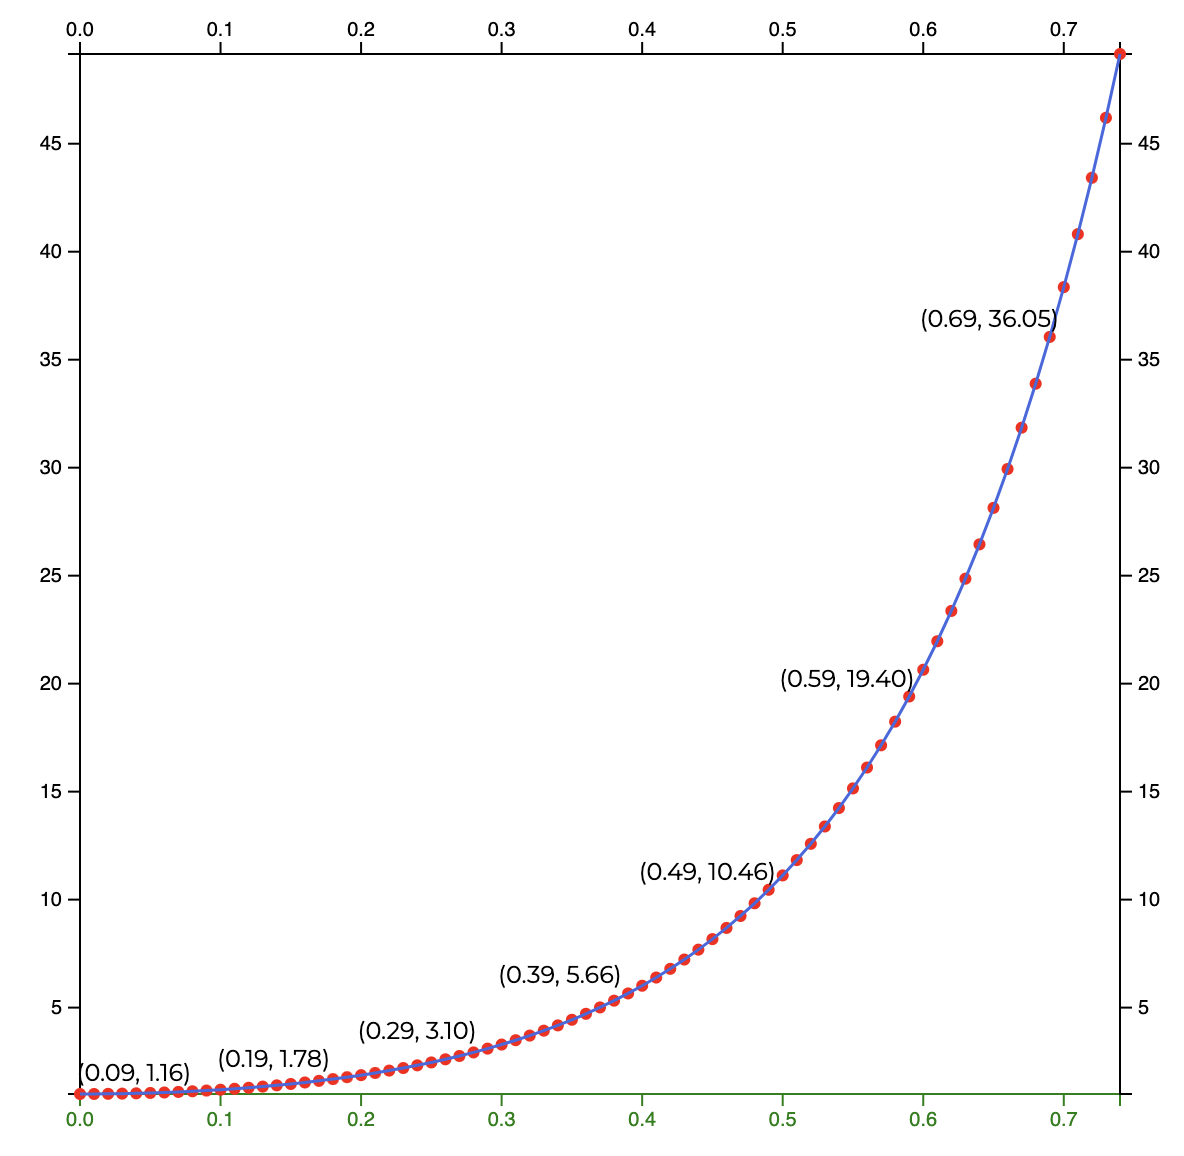
\includegraphics[width=0.75\textwidth]{data/ex27.png}
\caption{ A line chart with markers and data labels.}
\label{fig:ex27}
\end{figure}


\section{Part 14: Colorus}
\subsection{ Exercise 28 }
\vspace{-1em}
Exercise 28 required using a method to generate colour schemes to colour a bar chart based on its data values. A colour scheme was generated using the scaleSequential(), domain() and interpolator() functions. scaleSequential() generates a sequential scale to map continues values to an output, domain() specifies the accepted values (typically between the min and max value of the data provided) and the interpolator() which accepts a pre-defined function in D3 that returns a colour scale.



\subsection{Exercise 29 }
\vspace{-1em}
Exercise 28 required to generate a colour collection and use it to colour a line chart. A colour scheme was generated using the scaleLinear(), domain() and range() functions. scaleLinear() specifies a linear relationship between values in the domain and values in the range() species the range of the scale, and accepts colour as input variables, thus creating a colour scale, mapping each input value to a colour within this range (Figure \ref{fig:ex29}). The line is added as a single path therefore data markers are introduced to colour each individually based on the data value.

Using colour scales is useful in line charts with multiple lines to distinguish between the lines.

\begin{figure}[H]
\centering
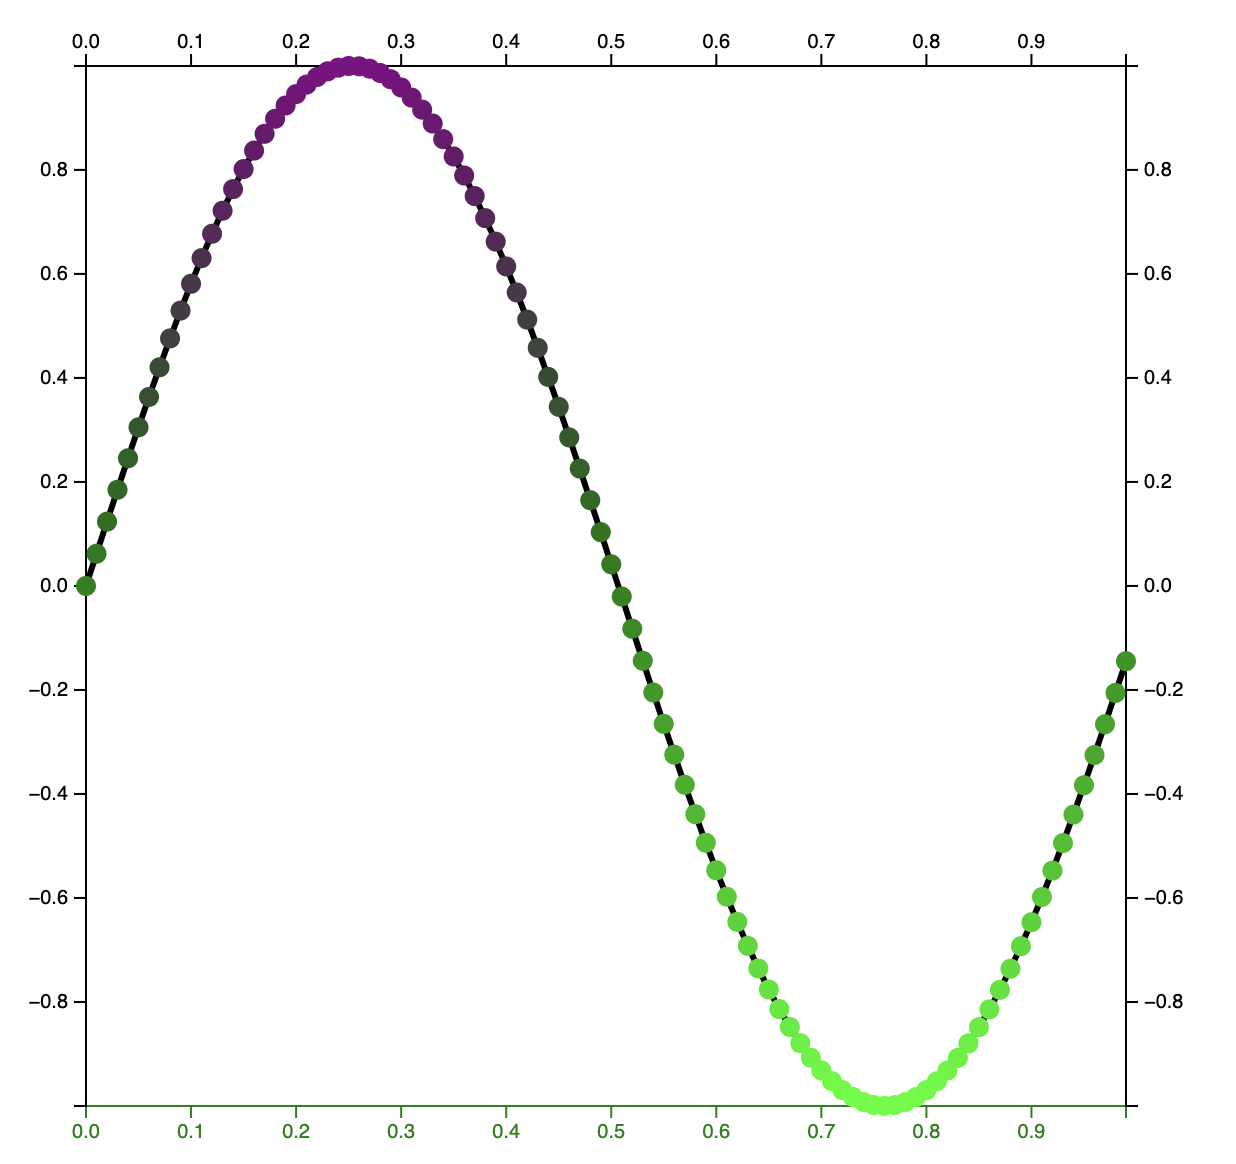
\includegraphics[width=0.75\textwidth]{data/ex29.png}
\caption{ A line chart with data markers coloured based on the y value.}
\label{fig:ex29}
\end{figure}


\section{Part 15: Pie Chart }
\subsection{Exercise 30}
\vspace{-1em}
Exercise 30 required expanding the example pie chart code given to include additional data values. A pie chart is constructed from data given in an array format therefore this is simply the case of adding additional datapoints to the data array. Creating a pie or donut chart requires the use of pie() and arc() functions. First, pie() is used which generates a JSON object per datapoint that contains the data value, its starting and ending angle of each data value and index (in order from largest to smallest value). Second, arc() generates an arcs for each datapoint using starting/ ending angles from the pie() function, in addition inner (donut charts) and outer radius is specified.

\subsection{ Exercise 31}
\vspace{-1em}
Exercise 31 required adding text labels to the pie chart from exercise 30. Text labels are associated with each <g> container contained an arc for the given datapoint. First, all <g> elements for the given pie chart are selected and data() function is used to associate data to the selected DOM elements. An array of JSON objects is provided as an argument to data() in the form of pie31(data) function. The text of the label is the data value itself, accessed via d.value, while the starting and ending angles are used to determine the location of the label via the centroid() function. 

\section{Part 16: SVG Graphics}
\subsection{ Exercise 32}
\vspace{-1em}

Exercise 32 required adding a background image to a graph from one of the previous exercises. For this purpose a simple line graph with a sine function display is chosen. An SVG object is created and appended to the page which functions as container to the different graph elements, including the background image. Height, width and position of the SVG object are specified using pre-defined variables, the same variables are later used to determine the size and placement of the background image. In order for the background to only cover the main are of the graph, SVG's margins are excluded from the image's size and taken into consideration when repositioning the image. The image is appended as an "svg:image" element to the SVG object and the location of the image in the local repository is specified using the "xlink:href" attribute.     

\section{Conclusions}
To conclude, the lab explored the basic concepts of visualisation graphics and a solid foundation of D3 to build on in future labs.


\end{document}  
